\chapter{Применение программной системы}
\label{part:examples}

В данной главе продемонстрированы примеры применения разработанных инструментальных средств  для решения практических задач. 

%-----------------------------------------------------------------------------------------
%---------------------Эксперименты, тестирование, сравнение------------------------------
%-----------------------------------------------------------------------------------------
\section{Назначение программной системы}
Разработанная система АДТ предназначена для поиска ЛВ в первопорядковом исчислении ПО--формул. Помимо установки того факта что формула является теоремой, имеются средства, которые в некоторых случаях устанавливают противоречивость исходной формулы (т.е. невыводимость её в исчислении ПО--формул). Входным языком представления формул может служить язык логики предикатов первого порядка, язык дизъюнктов и язык ПО--формул. Для первых двух языков взят формат библиотеки TPTP, для ПО--формул разработан формат близкий к используемому в систем КВАНТ Е.А.~Черкашина \cite{dissChe}. Система относится к 1 и 3 классу систем АДТ, согласно классификации приведенной во введении.




%==============================================================================
%=============================== ТЕСТИРОВАНИЕ И СРАВНЕНИЕ======================
%==============================================================================
\section{Тестирование и сравнение}

Тестирование системы проводилось на задачах из библиотеки TPTP (Thousands of Problems for Theorem Provers, www.tptp.org). Данная библиотека является де--факто стандартом для тестирования систем АДТ. На момент написания работы библиотека содержала свыше 20000 задач, формализованных на языке предикатов первого порядка (FOF: first-order formula), конъюнктивной нормальной формы (CNF: clause normal form), типизированные формулы первого порядка(TFF: typed first-order form), типизированные формулы высшего порядка (THF: typed higher-order form). Кроме того, все зарегистрированные в библиотеке TPTP системы являются самыми передовыми (``state-of-the-art systems'') современными системами АДТ, с которыми можно производить сравнение, на соответствие мировому уровню.

Все задачи классифицированы по следующим параметрам, а именно:
\begin{enumerate}
\item {Рейтинг.} Измеряется числом от 0.0 до 1.0. Задача с рейтингом 0.0 решается любой передовой системой АДТ, внесённой в библиотеку. Задача с рейтингом 1.0 ещё не была решена ни одной системой. Внесенные в библиотеку системы АДТ именуются как  самые передовые (``state-of-the-art systems''). Задачи с рейтингом от 0.04 уже относятся к классу сложных (``difficult''). Далее, говоря ``сложная задача'' будем иметь ввиду что задача обладает рейтингом от 0.04. Тестирование проведено по всем видам рейтинга от 0.0 до 1.0.
\item {Предметная область задачи.} Например, теоремы математического анализа (ANA), алгебры (ALG), геометрии (GEO), головоломки (PUZ), медицины (MED), и др. Всего на момент тестирования имелось 48 областей.
\item {Количественные характеристики формулы.} Например, количество предикатов, функциональных символов, наличие предиката равенства, общий объем формулы.
\item {Статус.} теорема (theorem), выполнима (satisfiable), невыполнима (unsatisfiable), неизвестно (unknown), открытая проблема (open), т.е. в принципе не решенная задача. Основное тестирование будем проводить по задачам статуса ``теорма''.
\item {Формализация.} Язык логики предикатов первого порядка (FOF), конъюнктивная нормальная форма (CNF) и др.  
\end{enumerate}

Отметим, что библиотека регулярно обновляется и пополняется новыми задачами, требующих решения. Включенные в библиотеку системы, предназначены для решения задач из определенных областей, например, только для CNF и FOF, для теорем, для выполнимых задач и пр. 

В данном раздле представлены примеры решения задач, описания и формулировки этих задач, формализации целей, сравнение с другими системами, зарегистрированными в TPTP, статистические данные о формулах. Даны комментарии по эффективности применяемых стратегий, проведены эксперементы с включением и отключением стратегий. Кроме того, даётся сводная информация о результатах тестирования и сравнения с другими система АДТ. С учетом того что решаются в основном первопорядковые теоремы статуса ``теорема'', сравнение проводится с 31 системой АДТ, предназначеных для данных классов задач. Таблицы решенных задач по некоторым предметным областям представлены в приложении, кроме того в приложении представлены задачи, взятые с чемпионата мира среди систем АДТ 2012 (CASC-J6) \cite{CASC}.



%================================================================
\subsection{Сводная информация о результатах тестирования и сравнения}

Решенные задачи по рейтингу.

\begin{longtable}[H]{|p{0.35\linewidth}|p{0.25\linewidth}|p{0.15\linewidth}|}
\hline
\textbf{Рейтинг} & \textbf{Всего задач} & \textbf{Решено} \\
%\hline
%Рейтинг 0.0--1.00 & 1221 & 677 \\
\hline
Рейтинг 0.0--0.03 & 192 & 171 \\
\hline
Рейтинг 0.04--0.20 & 435 & 373 \\
\hline
Рейтинг 0.21--0.32 & 128 & 75 \\
\hline
Рейтинг 0.33--0.49 & 115 & 44 \\
\hline
Рейтинг 0.5--0.67 & 223 & 21 \\
\hline
Рейтинг 0.68--0.92 & 72 & 5 \\
\hline
Рейтинг 0.93--1.0 & 56 & 0\\
\hline
\end{longtable}


Лучшие показатели по предметным областям.

\begin{longtable}[H]{|p{0.4\linewidth}|p{0.2\linewidth}|p{0.15\linewidth}|}
\hline
\textbf{Предметная область} & \textbf{Всего задач} & \textbf{Решено} \\
\hline
Геометрия (GEO) & 242 & 204 \\
\hline
Менеджмент (MGT) & 22 & 22 \\
\hline
Синтаксические (SYN) & 275 & 180 \\
\hline
Семантический веб (SWB) & 25 & 22 \\
\hline
\end{longtable}


Самые сложные задачи, из решенных.

\begin{longtable}[H]{|p{0.2\linewidth}|p{0.2\linewidth}|p{0.2\linewidth}|p{0.2\linewidth}|}
\hline
\textbf{Задача} & \textbf{Рейтинг} & \textbf{Время} & \textbf{Шагов} \\
%\hline
%LCL662+1.005 & 1.0 & 1.02 & 7772 \\
\hline 
LCL652+1.015 & 0.92 & 32.1 & 185253 \\
\hline
LCL656+1.020 & 0.92 & 1.24 & 845 \\
\hline
\end{longtable}



Максимальный рейтинг задач, которые удалось решить 0.92, т.е. практически достигнута максимальная планка сложности проблем. 




%================================================================
\subsection{Примеры решенных задач}

%==================
\paragraph{COM003+1}
Формулировка: ``The halting problem is undecidable'' (``Неразрешимость проблемы остановки'' \cite{turing}). Известная теорема о неразрешимости проблемы остановки машины Тьюринга: ``Даны описание алгоритма и его начальные входные данные, требуется определить, сможет ли выполнение алгоритма с этими данными завершиться когда-либо''. Алан Тьюринг доказал, что не существует общего алгоритма для решения проблемы остановки, т.е. проблема остановки неразрешима.

Формализация данной задачи в языке логики предикатов первого порядка (FOF) включает 5 формул и 55 атомов. На сайте библиотеки TPTP: www.tptp.org по номеру задачи можно увидеть её в формате FOF. Формализация её на языке ПО--формул представлена в приложении.

Рейтинг задачи: 0.33. Время решения: 0.005с. Количество шагов: 185. 

Для сравнения приведем таблицу времени решения данной задачи одними из лучших, внесенными в TPTP, системами АДТ:

\begin{longtable}[H]{|p{0.2\linewidth}|p{0.35\linewidth}|}
\hline
\textbf{Система АДТ} & \textbf{Время решения (секунд)}  \\
\hline
Vampire & 0.01 \\
\hline
iProver & 0.47 \\
\hline
leanCoP & 29.25 \\
\hline
EP & 104.45  \\
\hline
Zenon & 0.08 \\
\hline
\end{longtable}


Как видно, время решения задачи нашей системой лучше, чем время решения других систем АДТ.

При решении данной задачи использовались стратегии: ленивая конкретизация (ограничение 1), $4,1$--опровержение, разделение данных по базе. Подключение параллельных стратегий, хотя и возможно, поскольку формула имеет дизъюнктивные ветвления, но в данном случае неоправданно, поскольку накладные затраты на создание процессов, перекрывают полезное время вычислений.


%==============================
\paragraph{LCL640+1.005}
Формулировка: ``In K, formula with A4 and Dum leading to Dum, size 5''. Описание проблемы дано в \cite{SourceLCL}. Представляет собой проблему модальной логики, выраженную в языке логики предикатов первого порядка.

Формализация данной задачи в языке логики предикатов первого порядка (FOF) включает 1 формулу и 121 атом. При этом структура формулы довольно сложная: глубина узлов достигает 16 уровней, имеется множество дизъюнктивных ветвлений.

Рейтинг задачи 0.62. %И это задача с самым высоким рейтингом, которую смогла решить наша систма.

Время решения: 0.05с. Количество шагов: 821.

Для сравнения приведем таблицу времени решения данной задачи одними из лучших, внесенными в TPTP, системами АДТ:

\begin{longtable}[H]{|p{0.2\linewidth}|p{0.35\linewidth}|}
\hline
\textbf{Система АДТ} & \textbf{Время решения (секунд)}  \\
\hline
Vampire & 0.06 \\
\hline
iProver & 39.52 \\
\hline
EP & 174.46  \\
\hline
Zenon & 9.89 \\
\hline
\end{longtable}


Как видно, время решения задачи нашей системой лучше, чем время решения других систем АДТ. Кроме того, отметим, что больше половины систем АДТ вообще не смогли решить эту задачу.

При решении данной задачи использовались стратегии: ленивая конкретизация (ограничение 1), $14,4$--опровержение, разделение данных по базе. Подключение параллельных стратегий, хотя и возможно, поскольку формула имеет дизъюнктивные ветвления, но в данном случае неоправданно, поскольку накладные затраты на создание процессов, перекрывают полезное время вычислений.



%========================
\paragraph{SYN548+1}
Формулировка: $\Diamond \Box (\Box (p \vee \Box q) \Leftrightarrow \Box p \vee \Box q)$

Комментарий из библиотеки TPTP: Это проблема модальной логики, транслированная в язык логики предикатов 1-ого порядка (FOF).
Проблема легко решается системами АДТ для модальных логик, но трансляция этой задачи в язык логики предикатов 1-ого порядка является сложой задачей. Первопорядковая трансляция операторов $\Box$ и $\Diamond$ выглядит так:
               	$[\Box P]x := (\forall y R(x,y) \rightarrow [P]y)$ \\
               	$[\Diamond P]x := (\exists R(x,y) \& [P]y)$ \\
               	$[P]x := P(x)$ \\
$P$ это атом, где мы стартуем с некоторым первоначальным контекстом o (первочанальный мир), т.е. мы преобразуем формулу $P$ в $[P]o$.

Рейтинг 0.54. Время решения: 5.8с. Количество шагов: 82764.

Для сравнения приведем таблицу времени решения данной задачи одними из лучших, внесенными в TPTP, системами АДТ:

\begin{longtable}[H]{|p{0.2\linewidth}|p{0.35\linewidth}|}
\hline
\textbf{Система АДТ} & \textbf{Время решения (секунд)}  \\
\hline
Vampire & 0.02 \\
\hline
iProver & 1.71 \\
\hline
EP & 59.54  \\
\hline
Zenon & 12.07 \\
\hline
\end{longtable}

Как видно, имеются системы, решившие задачу как значительно быстрее, так и значительно медленнее. Отметим, что рейтиг задач 0.54 говорит о том, что более половины систем АДТ не могут найти решение вообще.

При решении данной задачи использовались стратегии: ленивая конкретизация (ограничение 1), $8,2$--опровержение, $8,1$--конкретизация, разделение данных по базе, агрессивное разделение термов.

%=======================
\paragraph{MSC014+1}
Данная задача интересна тем, что не является теоремой. Тем не менее, с использованием полной стратегии вывода (т.е. без использования ограничивающих стратегий), данный факт устанавливается, в силу запирания ДСВ.

Рейтинг 0.33. Время решения 0.0007с. Другие системы, устанавливают данный факт тоже со временем близким к 0.


%===============================================
\subsection{Крупные задачи}

Рассмотрим поведение системы при решении некоторых крупных задач, формализация которых превышает 100~Кб. Как правило, это задачи с формализацией очень большого количества аксиом, многие из которых не пригождаются в выводе, т.е. ответы на многие вопросы заведомо не приносят никакой пользы, более того, наоборот, захламляют вывод. Основной тактикой при решении таких задач является, во-первых, повсеместное использование экономии памяти, тщательное использование собранной статистики для удаления ненужных фактов и вопросов, и, во-вторых, использование знаний о задаче, для выявления заведомо плохих ветвей вывода.

\paragraph{CSR025+3}
Рейтинг 0.17. Время решения 1с. Для сравнения, Vampire 0.14c, EP 0.7c, iProver 1.5c.
Данная задача содержит 1 группу аксиом, включающую 8006 формул и 13036 атомов.

\paragraph{CSR064+3}
Рейтинг 0.58. Время решения 4.4с. Для сравнения, EP 0.24c, iProver 5.8c.
Формулировка: ``Which British company was taken over by BMW in 1994?''

Количество формул 10189. Количество атомов 10803.

\paragraph{PUZ068+2}
Задача относится к классу satisfiable.
Рейтинг 0.0. Время решения 4с. Для сравнения. Vampire 1.1c, iProver 1.7c, EP 1.8c.

Количество формул 10547. Количество атомов 23545.


%===============================================================
\subsection{Сравнение с системами АДТ ИДСТУ СО РАН}
Задача ``о паровом катке'', как демонстрация решения сложной задачи была представлена в диссертации Черкашина Е.А. \cite{dissChe}.
В библиотеке TPTP на данный момент она имеет три формализации PUZ031+1 (рейтинг 0.08), PUZ031+2 (рейтинг 0.04), PUZ031+3 (рейтинг 0.08), и попрежнему входит в число сложных задач.

Решение всех трёх вариантов осуществляется за 0.005 (близко к 0), 0.002 (близко к 0) и 0.4 секунды соответственно. Глубина вывода 19 (является минимально возможным выводом). Для сравнения, EP, Vampire, Otter, время близко к 0.01. 

То есть, заметно значительное повышение производительности, как с точки зрения количества шагов, так и с точки зрения затраченного времени.



%==========================================
\subsection{Комментарии по стратегиям}

%=============================
\paragraph{Ленивая конкретизация.}
Эффективность данной стратегии по сравнению с прямым перебором эрбранова универса, даже не поддается сравнению, поскольку второй вариант как правило не приводит вообще к решению задачи за приемлемое время. Наиболее важную роль, в данной стратегии, играют ограничения, позволяющие значительно сокращать число шагов вывода по сравнению с использованием данной стратегии без ограничений. Сокращение числа шагов вывода, в данном случае, влечет и сокращение времени решения. Неформально, по степени важности данный подход мы ставим на первое место.


%===========================
\paragraph{Экономия памяти.}
Использование ДСВ, позволило реализовать многие другие стратегии и одновременно с этим экономить память разделяя общие данные ветвящихся формул. Агрессивное разделение данных и удаление излишек, позволило применить систему для решения некоторых задач с крупной формализацией, а стратегия выбора ответа приводящего к формуле с наименьшим весом, позволило максимально оттянуть момент достяжения лимита выделенной памяти. Для некоторых задач, например SYN548+1, указанной выше, снятие запрета на использование повторов подстановок, приводит к десятикратному повышению времени решения задач.

%=============================
\paragraph{$k,m$-ограничения.}
Эффективность данной стратегии, проявляется в задачах с дизъюнктвиынм ветвлением. Во всех случаях уместного использования данной стратгии и правильно выбранных параметров, достигает заметное повышение эффективности. Кроме того, данный подход позволяет реализовать полный перебор пространства поиска, что позволило найти для некоторых задач минимальный вывод.

%===========================
\paragraph{Параллельные стратегии.}
Важным свойством параллельных схем алгоритмов является их масштабируемость, т.е. степень повышения эффективности с увеличением количества вычислительных элементов (ВЭ). Поэтому основной характеристикой является не конкретное время исполнения программ, а соотношение времени исполнения программы в параллельном режиме на заданном количестве ВЭ к времени исполнения этой же программы на одном ВЭ при различном количестве ВЭ.

Эксперименты проводились на задачах, формализация которых в языке ПО--формул обладает необходимыми свойствами для испытания параллельных стратегий, а именно: дизъюнктивное ветвление, большое количество вопросов, крупные конъюнкты вопроса. Результаты находятся в соответствии с представленной иерархией стратегий. На рис. \ref{fig:parallel} представлены результаты данного тестирования.
\begin{figure}[h]
	%\vspace{0.5cm}
	\centering
	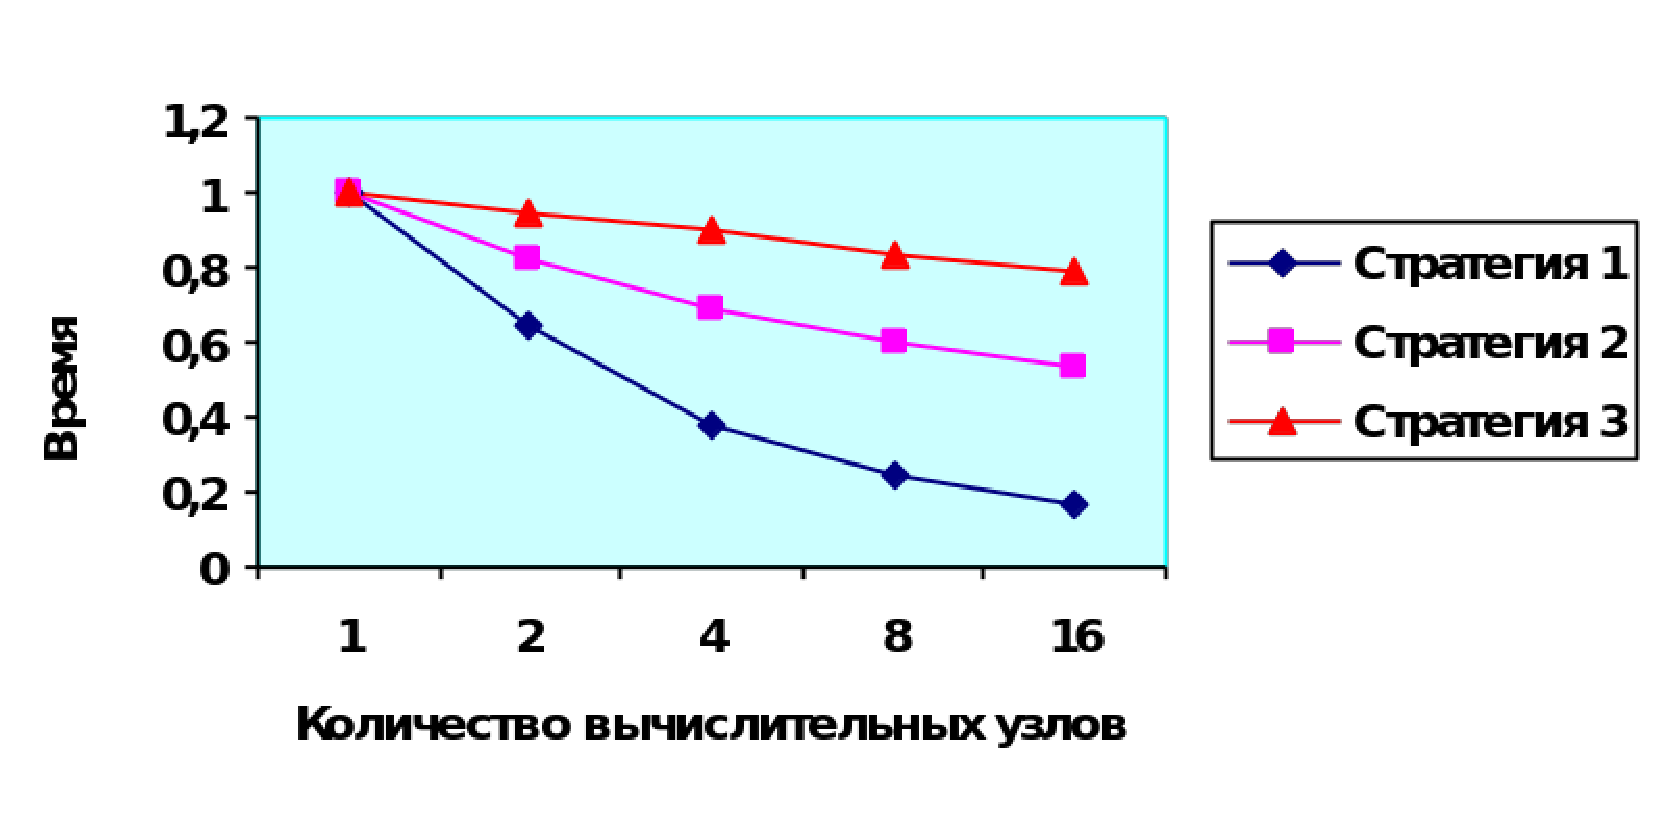
\includegraphics[width=0.7\linewidth]{pics/Parallel.eps}
	\caption{Результаты тестирования параллельной реализации алгоритмов АДТ, согласно представленной стратегии}
	\label{fig:parallel}
\end{figure}

Наибольшую эффективность, как и следовало ожидать, показала первая стратегия, естественно при наличии дизъюнктивного ветвления в исходной формуле. Под эффективностью понимается уменьшение затрачиваемого времени с увеличением количества вычислительных узлов.


%===========================
\paragraph{Равенства.}
Стратегия генерации эквивалентных атомов в базе, хотя и даёт принцпиальное опровержение формулы, и повышение эффективности по сравнению с прямым использованием аксиом равенства, тем не менее, как правило, проигрывает другим системам АДТ при решении задач с равенствами. Однако, использование такого подхода, обусловлено желанием сохранить основные положительные свойства ПО--формул.

%===========================
\paragraph{Менеджер памяти и кэширование.}
Помимо использования стратегий из главы~\ref{part:two}, значительные результаты в повышении эффективности поиска ЛВ достигнуты благодаря использованию менеджера памяти и кэширования результатов.

%=============================================================================
%=========================ВЫВОДЫ================================================
%=============================================================================
\section{Выводы}
Система протестирована на разных классах задач, в основном взятых из библиотеки TPTP.  

Тестирование решенных задач, подтвердило предположение авторов исчисления ПО--формул, о том что крупноблочная структура формул и правила вывода позволяет повысить эффективность поиска ЛВ. Задачи, формализация которых в языке ПО--формул обладает свойством крупноблочности, а именно больших конъюнктов, решаются более эффективно, в сравнении с другими системами АДТ. Кроме того, наблюдается небольшой выигрыш в задачах, формализация которых в языке ПО--формул, включает экзистенциальные переменные и глубокие вопросы. Все перечисленные свойства: крупноблочность, явное использование двух видов кванторов, сохранение исходной структуры знания, являются основными отличительными свойствами от резолютивных методов. Продемонстрирована эффективность данных отличий.

С точки зрения предметных областей, наилучшая эффективность системы показана на задачах геометрии, менеджмента, семантического веба, и некоторых других.

Рейтинг решенных задач варьируется от 0.0 до 0.92 (с учетом того что сложные задачи начинаются от рейтинга 0.04), т.е. решаются, в том числе сложнейшие задачи библиотеки TPTP, в том числе многие из них более эффективно чем другими лучшими системами АДТ. Выигрыши по сравнению с ними выражается меньшим временем или количеством шагов вывода. Таким образом, делается вывод, что разработанная система соответствует мировому уровню.

Манипуляцию с включением и отключением стратегий наглядно показывают, что они положительно влияют на эффективность поиска ЛВ. То есть, подтверждено на практике положительное влияние предложенных стратегий повышения эффективности поиска ЛВ.

Ещё одним результатом является значительное расширение класса решаемых задач по сравнению с предыдущими системами АДТ базирующимися на исчислении ПО--формул. Для раннее решаемых задач не только повышена эффективность их решения, но и достигнуты некоторые пределы эффективности, в частности найден минимальный вывод некоторых задач.

Лучшие системы, включенные в библиотеку TPTP имеют приоритет при решении задач содержащих много предикатов равенства.




%=================
%\paragraph{SWB020+2}
%Рейтинг 0.5. Время решения 0.04 секунды. Для сравнения, EP 0.01с, Vampire 0.01с, iProver 10c.

%Формализация занимает 60 атомов и 8 подформул--вопросов. Формализация в языке ПО--формул занимает 5~кб, и представлена в приложении.




%==================
%\paragraph{SYN353+1} Рейтинг задачи 0.54.
%Разработанная система решает её за 33 шага, без учета стратеги k,m-ограничений, т.е. фактически шагов может быть больше, но %глубина окончательного вывода 33. Затраченное время 1.1с. Для сравнения, Vampire решает эту задачу за 0.7с, SPASS за 0.78с, Prover9 за 4.0с.

%Задача взята из книги \cite{Church1}, где имеет номер  46.18 (5). В формате FOF TPTP формализуется следующим образом:

%\begin{quote}
%\texttt{\raggedright\noindent
%fof(church\_46\_18\_5,conjecture,\\
%~~~~(~!~[X]~:\\
%~~~~~~?~[Y1,Y2,Y3]~:\\
%~~~~~~!~[Z]~:\\
%~~~~~~~~(~(~big\_f(Y1,Y2,Y3)\\
%~~~~~~~~~=>~(~big\_f(X,X,Z)\\
%~~~~~~~~~~~=>~(~big\_f(Y2,Y3,Y1)\\
%~~~~~~~~~~~~~~|~big\_f(Y3,Y1,Y2)~)~)~)\\
%~~~~~~~=>~(~(~(~big\_f(Y3,Y1,Y2)\\
%~~~~~~~~~~~~~=>~(~big\_f(Y1,Y2,Y3)\\
%~~~~~~~~~~~~~~~~\&~big\_f(Y2,Y3,Y1)~)~)\\
%~~~~~~~~~~<=>~big\_f(Y2,Y1,Z)~)\\
%~~~~~~~~~=>~(~(~(~big\_f(Y2,Y3,Y1)\\
%~~~~~~~~~~~~~~~=>~(~big\_f(Y1,Y2,Y3)\\
%~~~~~~~~~~~~~~~~~~~big\_f(Y3,Y1,Y2)~)~)\\
%~~~~~~~~~~~~<=>~big\_f(Y1,Z,Y2)~)\\
%~~~~~~~~~~~=>~(~(~(~(~big\_f(Y3,Y1,Y2)\\
%~~~~~~~~~~~~~~~~~~~=>~\~~big\_f(Y2,Y3,Y1)~)\\
%~~~~~~~~~~~~~~~~~=>~big\_f(Y1,Y2,Y3)~)\\
%~~~~~~~~~~~~~~<=>~big\_f(Z,Y2,Y1)~)\\
%~~~~~~~~~~~~~=>~(~(~big\_f(Y1,Y2,Y3)\\
%~~~~~~~~~~~~~~~~~~\&~big\_f(Y2,Y3,Y1)\\
%~~~~~~~~~~~~~~~~~~\&~big\_f(Y3,Y1,Y2)~)\\
%~~~~~~~~~~~~~~<=>~big\_f(Z,Z,Z)~)~)~)~)~)~)).}
%\end{quote}


%LCL631+1.005
%\paragraph{LCL636+1.005}
%Рейтинг 0.5. Время решения 5 секунд. Количество шагов 20, без учёта возможных возвратов. Для сравнения, EP 0.5c, Vampire 1.2c, iProver 8c, Prover9 13c.

%Формулировка: ``The branching formula plus a negation symbol in front and an additional subformula to make the formula provable''.
%Взято из статьи \cite{SourceLCL}.

%Формализация включает 719 атомов и 1361 логическую связку.


%LCL640+1.005
%\paragraph{LCL640+1.005}
%Рейтинг 0.62. Время решения 0.4 секунды. Количество шагов 130, без учёта возможных возвратов. Для сравнения, Vampire 0.1с, SPASS 9с, iProver 35c, EP 98c.

%Формализация включает 121 атом и 236 логических связок.

%SYN723+1; рейтинг 0.5; на этапе трансляции
%\paragraph{SYN723+1}
%Рейтинг 0.5. Решается на этапе трансляции и редукции формулы, т.е. приводится к виду $\forall: True \exists: False$.

%\paragraph{SYN548+1}
%Рейтинг 0.54. Время решения 0.01 секунды. Количество шагов 80. Для сравнения, EP 0.01c, Vampire 0.01c, iProver 0.01c.

%Проблема модальной логики \cite{chellas}, представленная в языке логики предикатов первого порядка.
%LCL652+1.005
%\paragraph{LCL652+1.005}
%рейтинг 0.79. решает быстро..

%Рассмотрим более подробную информацию о задачах из геометрии и сравнении с другими системами. Полный список решенных задач представлен в приложении.

%\paragraph{GEO205+3}
%Рейтинг 0.33. Время решения 0.08. Количество шагов 12. Для сравнения, Ayane 0.26c, Vampire 0.42c, EP 1.63c.

%Формалуировка: ``If the lines X and Y are convergent, and Y and Z are  equivalent, then X and Z are convergent, and the intersection   point of X and Y, and the intersection point of X and Z are equal''.
%\begin{quote}
%\texttt{\raggedright\noindent
%fof(con,conjecture,(\\
%~~~~!~[X,Y,Z]~:\\
%~~~~~~(~(~convergent\_lines(X,Y)\\
%~~~~~~~~\&~equal\_lines(Y,Z)~)\\
%~~~~~=>~(~convergent\_lines(X,Z)\\
%~~~~~~~~\&~equal\_points(intersection\_point(X,Y),\\
%~~~~~~~~~~~intersection\_point(X,Z))~)~)~)).\\
%~~~~~~~~}
%\end{quote}
%При этом используется 7 групп аксиом, общий объём которых в языке ПО--формул составляет 5~кб.

%----------------------------------------------
%\paragraph{GEO222+3.p}
%Рейтинг 0.17. Время решения 0.01с. Количество шагов 27. Для сравнения, EP 0.03c, Vampire 0.03c, Otter 0.5c, Prover9 0.6c.

%Формулировка задачи: ``A line L is parallel to the line, that is orthogonal to the orthogonal to L through A, and goes through A as well''.

%Формализация цели следующая:
%\begin{quote}
%\texttt{\raggedright\noindent{}fof(con,conjecture,(\\
%~~~~!~[A,L]~:~parallel\_lines(L,\\
%~~~~~~~~~orthogonal\_through\_point(\\
%~~~~~~~~~~~~~orthogonal\_through\_point(L,A),A))~)).}
%\end{quote}
%При этом используется 7 групп аксиом, общий объём которых в языке ПО--формул составляет 5~кб.

%----------------------------------------------
%\paragraph{GEO264+1}
%Рейтинг 0.04. Время решения 0.005с. Для сравнения, Ayane 0.01c, Vampire 0.01, iProver 0.04c.

%Формулировка: ``Triangle divides plane into seven regions''.

%Формализация цели:
%\begin{quote}
%\texttt{\raggedright\noindent
%fof(con,conjecture,(\\
%~~~~!~[A,B,C,D]~:\\
%~~~~~~(~left\_apart\_point(C,line\_connecting(A,B))\\
%~~~~~=>~(~(~left\_apart\_point(D,reverse\_line(line\_connecting(B,C)))\\
%~~~~~~~~~~\&~left\_apart\_point(D,reverse\_line(line\_connecting(C,A))))\\
%~~~~~~~=>~left\_apart\_point(D,line\_connecting(A,B))~)~)~)).}
%\end{quote}
%Используется набор аксиом GEO007+0 из \cite{constrgeo}.

%----------------------------------------------
%006, 008

%\paragraph{MGT006+1}
%Рейтинг 0.12. Время решения 0.01с. Для сравнения, Vampire 0.01c, EP 0.05c.

%Формулировка: ``Reliability and accountability increase with time.''.

%\paragraph{MGT036+1}
%Рейтинг 0.12. Время решения 0.05с. Для сравнения, Vampire 0.01c. EP 0.01, Ayane 3.2c.

%Формулировка: ``First movers never outcompete efficient producers.''.

%\paragraph{MGT022+2}
%Рейтинг 0.04. Время решения 0.002с. Для сравнения, Vampire 0.01c, EP 0.01c, Ayane 3.1c.

%Формулировка: ``Decreasing resource availability affects the disbanding rate of first movers more than the disbanding rate of efficient producers.''.


%===============================================================
%\subsection{Задача из медицины}
%Основным источником формализации задач медицины является работа \cite{med1}.

%\paragraph{MED002+1}
%Рейтинг 0.38. Время решения 0.04с. Для сравнения, Vampire 0.01c, iProver 0.04c, SPASS 6.78c.

%Формулировка: ``Whether or not patients with nearly-exhausted production of glucose in the B-cells are cured with a biguanide and sulfonylurea combination therapy''.

%Формализация цели:
%\begin{quote}
%\texttt{\raggedright\noindent{}fof(treatmentne,conjecture,\\
%~~~~(~(~!~[X0]~:\\
%~~~~~~~~~~(~\~~gt(n0,X0)\\
%~~~~~~~~~=>~(~drugbg(X0)\\
%~~~~~~~~~~~~\&~drugsu(X0)~)~)\\
%~~~~~~\&~!~[X0]~:\\
%~~~~~~~~~~(~gt(n0,X0)\\
%~~~~~~~~~=>~conditionhyper(X0)~)\\
%~~~~~~\&~bcapacityne(n0)~)\\
%~~~=>~!~[X0]~:\\
%~~~~~~~~(~\~~gt(n0,X0)\\
%~~~~~~~=>~conditionnormo(X0)~)~)).}
%\end{quote}

%При этом используется следующий набор аксиом MED001+0, включающий в себя 18 формул.

%-------------------------------------
%\paragraph{MED009+1}
%Рейтинг 0.54. Время решения 1.9c. Для сравнения, Vampire 1.2c, EP 14c, SPASS 18.7c.

%Формулировка: ``After unsuccessful treatment with single oral anti-diabetic for patients with QI greater equal than 27 medical management moves to next step.''

%Формализация цели:
%\begin{quote}
%\texttt{\raggedright\noindent{}
%fof(transs1s2\_qige27,conjecture,\\
%~~~~(~(~s1(n0)\\
%~~~~~~\&~!~[X0]~:\\
%~~~~~~~~~~(~gt(n0,X0)\\
%~~~~~~~~~=>~conditionhyper(X0)~)\\
%~~~~~~\&~\~~bcapacitysn(n0)\\
%~~~~~~\&~\~~qilt27(n0)~)\\
%~~~=>~?~[X0]~:\\
%~~~~~~~~(~\~~gt(n0,X0)\\
%~~~~~~~~\&~s2(X0)\\
%~~~~~~~~\&~!~[X1]~:\\
%~~~~~~~~~~~~(~gt(X0,X1)\\
%~~~~~~~~~~~=>~conditionhyper(X1)~)\\
%~~~~~~~~\&~(~bcapacityne(X0)\\
%~~~~~~~~~~|~bcapacityex(X0)~)~)~)).}
%\end{quote}

%Используется две группы аксиом MED001+1 и MED001+1.

%-------------------------------------
%\paragraph{MED010+1}
%Рейтинг 0.46. Время решения 3.1 секунды. Для сравнения, iProver 0.05c, Vampire 0.05c, EP 6c.

%Формулировка: ``After unsuccessful treatment with two oral anti-diabetic medical management moves to next step''.

%Формализация цели в FOF формата TPTP выглядит так:
%\begin{quote}
%\texttt{\raggedright\noindent{}fof(unsuccesfuls2,conjecture,
%~~~~(~(~s2(n0)\\
%~~~~~~\&~!~[X0]~:\\
%~~~~~~~~~~(~gt(n0,X0)\\
%~~~~~~~~~=>~conditionhyper(X0)~)\\
%~~~~~~\&~bcapacityex(n0)~)\\
%~~~=>~?~[X0]~:\\
%~~~~~~~~(~~~gt(n0,X0)\\
%~~~~~~~~\&~s3(X0)\\
%~~~~~~~~\&~!~[X1]~:\\
%~~~~~~~~~~~~(~gt(X0,X1)\\
%~~~~~~~~~~~=>~conditionhyper(X1)~)\\
%~~~~~~~~\&~bcapacityex(X0)~)~)).}
%\end{quote}

%При это используется две группы аксиом: MED001+0 (18 формул) и MED001+1 (22 формулы).



%=========================================================
%\subsection{Задачи верификации}


%===============================================================
%\subsection{Задачи головоломки}
%PUZ031+1
%20 шагов
%0.08с


%===============================================================





%===============================================================
%\subsection{Разное}

%Задачи которые стоит посмотреть:
%SYN457+1.p

%Из решенных задач время быстрее чем у Otter. Оттер выводит системную инфу всякую, поэтому думаю сопоставимо время на самом деле.

%Задача; Рейтинг; Статус (Решил ли прувер); Комментарий.

%ALG211+1; 0.12; Теорема (Да); 0.05 и 40 шагов.
%GRA014; 0.00; Теорема (Да); 1.2с и 5201 шагов. У Otter уходит 7 секунд. При этом вывод системной инфы не такой огромный.
%SET913+1; 0.04; ..


%Новое
%\paragraph{MSC010+1}
%Рейтинг 0.33. Время решения 0.03с. Количество шагов 812. Для сравнения, EP 0.01, Vampire 0.5c, iProver 3.8c.

%Формулировка: ``Verification of the negation of a conjecture, which is simply to prove the double negated version of a formula from the formula''.

%Формализация включает 136 атомов.


%------------
%MSC011+1; 7, 0.0002; 0.0
%MSC012+1; 48, 0.02; 0.12

%----------------------
%\paragraph{MSC014+1}
%Рейтинг 0.33. Время решения 0.0007с. Для сравнения, EP, Vampire, iProver все близко к 0.

%Задача является satisfiable.



%В некоторых случаях, включение параллельного режима вызывает обратный эффект, т.е. замедление, это связано с тем что решаемая задача сама по себе достаточно проста, а  накладные расходы связанные с созданием дополнительных процессов, копирования данных и т.д. превышает полезный ресурс направленный на опровержение баз.

%Сравнение с иными системами АДТ, показывает что разработанная система выигрывает по времени чаще всего при решении таких задач, формализация которых содержит достаточно объёмные конъюнкты, экзистенциальные переменные и глубокие вопросы.

%Значительный прирост эффективности достигается за счёт кэширования результатов. Опыты показывают что во время поиска ЛВ производится множество дублирующихся шагов и добавление повторяемой информации.


%Как видно, каждый узел дерева состояний вывода отождествляется с шагом вывода. Кроме того, узел содержит очень много дополнительной информации, т.е. потребляет ресурсы памяти, причем с каждым шагом вывода потребление может увеличиваться. Таким образом с точки зрения потребления ресурсов прувер эффективнее использовать на задачах имеющих крупноблочную структуру, т.е., при формализации конъюнкты действительно должны быть конъюнктами, а не вырожденными одноэлементными или пустыми, древовидная структура действительно должна быть древовидной, глубокой, а не с глубиной 4. Таким образом получится что каждый узел будет “обслуживать” довольно объемные и информативные куски данных. Одновременно с этим язык ПО--формул как раз и позиционируется как крупноблочный. Отсюда предположительно успех может возникнуть в задачах, формализуемых в языке ПО--формул таким образом, чтоб как можно сильнее проявлялась крупноблочность. %В самой крупной библиотеке формализованных задач из 10000 задач оказалось что 2000 обладают этим свойством. Поэтому тестирование и сравнение будет проводиться в следующих выборках: задачи которые предположительно наиболее удачно подходят для нашего прувера; и задачи которые предположительно являются неподходящими.

%С другой стороны задачи с неограниченными переменными приводят к использования стратегии ленивой конкретизации, что в конечном итоге может усложнить прозрачность логического вывода. Отсюда к перечисленным выше выборкам будут добавлены задачи с ограниченным и неограниченными переменными.




%%% Local Variables:
%%% mode: latex
%%% TeX-master: "dis"
%%% End:
